\chapter{SAGE}


SAGE és un software de que càlcul matemàtic que busca ser una alternativa oberta a Maple, Mathematica, Magma o MATLAB. Té paquets d'àlgebra, geometria, teoria de nombres, criptografia, computació numèrica i altres àrees. Ofereix una closca per sobre de software como Maxima, NumPy, SciPy, Octave, etc i l'implementa amb Python. D'aquesta manera junta el software existent per tal d'oferir-lo d'una manera única. Inicialment va ser creat per a recerca en matemàtiques i actualment utilitzat també per docència. Ens centrarem en el quadern de SAGE tot i que la instal·lació també inclou una terminal.



\section{Algunes propietats}

En el quadern no hem d'importar mòduls tal i com requeríem amb la llibreria \emph{math}, tot i que sí que podem importar els mòduls de Python com Numpy. Donat que SAGE integra diversos paquets, també permet l'execució de diversos llenguatges. Per exemple podem implementar \emph{scripts} en llenguatge Bash especificant abans de la cel·la l'interpret escrivint {\tt \%sh} o seleccionant el llenguatge al menú d'intèrprets.


\begin{blockcode}
%sh
for i in {1..10}; do echo $i; done
\end{blockcode}

Si volem especifica SAGE podem escriure {\tt \%sage}.

\begin{blockcode}
%sage
print("codi en sage")
\end{blockcode}


SAGE inclou l'autocompletat. Si anem al quadern, assignem una variable, després introduïm un punt per accedir els mètodes i premem la tecla {\tt Tab} veurem totes les possibilitats. Per exemple el mètode {\tt .N()} ens tornarà el valor numèric. Aquesta opció serà útil degut a que SAGE ens retornarà sempre que pugui la forma simbòlica de les nostres operacions.


\begin{blockcode}
sage: x = 4
sage: x.
\end{blockcode}


Al igual que amb Python podem obtenir més informació d'una element afegit el símbol {\tt ?} al final com es mostra a la Fig. ~\ref{fig:shelp}.



\begin{figure}[!h]
    \begin{centering}
    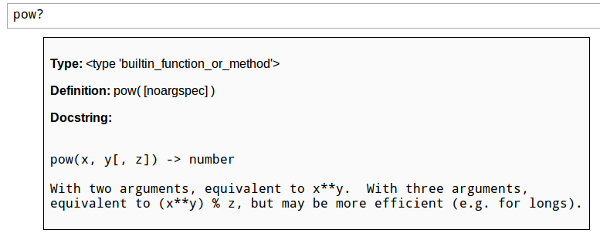
\includegraphics[width=0.9\textwidth]{img/shelp.png}
    \caption{Ajuda d'un mètode de SAGE}
    \label{fig:shelp}
    \end{centering}
\end{figure}

Els operadors són els mateixos. En el cas d'una divisió en la que perdi precisió en el resultat la deixarà en forma de fracció. Els operadors $**$ i $\wedge$ són equivalents

\begin{blockcode}
sage: 2*3
6
sage: (2+3j)-(4-8.3j)
-2.00000000000000 + 11.3000000000000*I
sage: 3//2
1
sage: 238/4
119/2
sage: 236/2
118
sage: 3**10
59049
sage: 3^10
59049
sage: 10%3
1
\end{blockcode}

Com veiem SAGE també realitza conversions implícites de tipus. Procurarà reduir les expressions fins que no en sàpiga més tal i com veiem amb les fraccions.

Hi han funcions que seran membre de la variable que té el valor tal i com la comprovació de nombres prims o la factorització, però el càlcul del màxim comú divisor ({\tt gcd}) serà una funció a part.

\begin{blockcode}
sage: x = 3
sage: x.is_prime()
True
sage: y = 1001
sage: y.factor()
7 * 11 * 13
sage: gcd(123213,432432)
3
\end{blockcode}

Entre les funcions comuns ens trobem l'arrodoniment. La funció {\tt floor()} arrodoneix a la baixa i {\tt ceil()} a l'alça.

\begin{blockcode}
sage: floor(3.9)
3
sage: ceil(3.1)
3
\end{blockcode}

Trobarem funcions trigonomètriques com {\tt cos, sin atan}, etc, o altres funcions comuns com {\tt sqrt} incloses també dintre de la llibreria {\tt math} de Python, però en aquest cas hi podem accedir directament. En el cas de la trigonometria també entén les correspondències a fraccions tal i com el cas.

\[
sin(\frac{\pi}{3}) = \frac{1}{2}\sqrt{3}
\]

\begin{blockcode}
sage: sin(pi/3)
1/2*sqrt(3)
\end{blockcode}



En el cas de SAGE considera tan el logaritme com el logaritme neperià amb base $e$ que és a la vegada una constant definida en l'entorn. Per a poder utilitzar una base diferent s'ha d'especificar com a segon paràmetre

\begin{blockcode}
sage: ln(e)
1
sage: log(e)
1
sage: log(125,5)
3
\end{blockcode}




\section{Solucionar equacions}

Quan volem una igualtat i no una assignació a SAGE utilitzarem l'operand lògic de Python $==$. Per a poder utilitzar una variable per a resoldre equacions haurem d'inicialitzar-la emprant la funció {\tt var()}. Quan volem fer que una variable de funció deixi de ser-ho utilitzem la funció {\tt restore()}

\begin{blockcode}
sage: 9 == 9
True
sage: 9 <= 10
True
sage: x = var("x")
sage: 3*x - 10 == 5
3*x - 10 == 5
sage: restore('x')
\end{blockcode}

SAGE procurarà retorna-nos el resultat de l'expressió en forma simbòlica abans que solucionar en una forma numèrica del conjunt real.

\begin{blockcode}
sage: solve( cos(x) - exp(x) == 0 , x)
[cos(x) == e^x]
sage: solve( exp(x) - x == 0 , x)
[x == e^x]
\end{blockcode}

En el cas de que vulguem una solució numèrica haurem de passar com a paràmetre l'equació i un interval on trobar l'equació.


\begin{blockcode}
sage: find_root(sin(x) == x, -pi/2 , pi/2)
0.0
sage: find_root(sin(x) == cos(x), pi, 3*pi/2)
3.9269908169872414
\end{blockcode}

Podem utilitzar la funció {\tt solve()} també amb diverses variables de la funció.

\begin{blockcode}
sage: y = var("y")
sage: solve( [3*x - y == 2, -2*x -y == 1 ], x,y)
[[x == (1/5), y == (-7/5)]]
\end{blockcode}


\section{Funcions}

En SAGE també tenim funcions matemàtiques a part de les funcions que em vist a programació. Podem definir funcions de la següent forma i detectarà quin tipus de funció declarem.


\begin{blockcode}
sage: f(x) = x*exp(x)
sage: f
x |--> x*e^x
sage: g(x) = (x^2)*cos(2*x)
sage: g
x |--> x^2*cos(2*x)
sage: h(x) = (x^2 + x - 2)/(x-4)
sage: h
x |--> (x^2 + x - 2)/(x-4)
\end{blockcode}

Els caràcters {\tt |--> } ens diuen que ens trobem amb una funció. Per cridar aquestes funcions les cridem amb el paràmetre numèric.

\begin{blockcode}
sage: f(1)
e
sage: g(2*pi)
4*pi^2
sage: h(-1)
2/5
\end{blockcode}



Podem avaluar límits de funcions passant com a primer paràmetre el nom de la funció i com a segon el valor pel qual volem avaluar.



\begin{blockcode}
sage: limit(f, x=1)
e
sage: limit(g, x=2)
4*cos(4)
sage: limit(h, x = 4)
Infinity
\end{blockcode}

També podem donar valor infinit a l'hora d'avaluar els límits.

\begin{blockcode}
sage: i(x) = x/x
sage: limit(i, x = Infinity)
1
\end{blockcode}

També podem avaluar el límit per la dreta o l'esquerra d'una funció


\begin{blockcode}
sage: limit(h, x=4, dir="right")
+Infinity
sage: limit(h, x=4, dir="left")
-Infinity
\end{blockcode}


Per a realitzar gràfics utilitzarem la funció {\tt plot} i per a mostrar els resultat cridarem a la funció {\tt show}. El resultat l'hem de recollir en un objecte. Implícitament estarem utilitzant llibreries gràfiques com GnuPlot, matplotlib, openmath o surf.


\begin{blockcode}
f(x) = sin(x)
p = plot(f(x), (x, -pi/2, pi/2))
p.show()
\end{blockcode}

Al igual que en Matplotlib podem acumular resultats. En aquest cas haurem d'utilitzar l'operand {\tt +} per a ajuntar els resultats.

\begin{blockcode}
sage: f(x) = sin(x)
sage: g(x) = cos(x)
sage: p = plot(f(x),(x,-pi/2,pi/2), color='black')
sage: q = plot(g(x), (x,-pi/2, pi/2), color='red')
sage: r = p + q
sage: r.show()
\end{blockcode}

Pot realitzar plots paramètrics on declarem una funció i l'interval d'aquesta funció
\begin{blockcode}
t = var('t')
p = parametric_plot( [3*cos(t), 3*sin(t)], (t, 0, 2*pi) )
p.show()
\end{blockcode}


\section{Programació}

Al igual que en Python ens trobem les estructures llista o diccionari. També trobem funcions pròpies de Python i mètodes dels elements que ens permeten interactuar amb les estructures de dades.

\begin{blockcode}
sage: d = {'1':True,'0': False}
sage: d['1']
True
sage: l = [3,5,1,3,5,2]
sage: l[2]
1
sage: len(l)
6
sage: type(l)
<type 'list'>
sage: l.count(5)
2
\end{blockcode}

De la mateixa manera que en altres llenguatges com Bash, podem crear llistes donant un interval de nombres naturals i introduint dos punts entre mig.

\begin{blockcode}
sage: m = [1..10]
sage: m
[1, 2, 3, 4, 5, 6, 7, 8, 9, 10]
sage: 3 in [1..10]
True
\end{blockcode}


Podem utilitzar funcions que treballen amb llistes tal i com vam veure amb NumPy

\begin{blockcode}
sage: sum([1,2,3])
6
sage: sum([1..100])
5050
sage: prod([1..4])
24
\end{blockcode}

I les funcions especials com {\tt map} o {\tt filter} estan implementades, al igual que les funcions anònimes lambda.

\begin{blockcode}
sage: map(lambda x: x^x, [1..9])
[1, 4, 27, 256, 3125, 46656, 823543, 16777216, 387420489]
\end{blockcode}

Les operacions condicionials es declaren igual.

\begin{blockcode}
z = 3
if z == 2:
    print "Dos"
else:
    print "no es tres"
\end{blockcode}
    
Podem declarar també els bucles {\tt for} i {\tt while} com fèiem amb Python.    

\begin{blockcode}
for i in [0..3]:
    sin(float(i))
\end{blockcode}



Les funcions venen implementades igualment per per Python.


\begin{blockcode}
def fun(x):
    print(log(x))
fun(e)
\end{blockcode}


\subsubsection*{Exercici \Roman{exercici}} \stepcounter{exercici}

Per a provar SAGE el que farem serà hackejar una clau privada. A la criptografia actual la seguretat es basa en que és costosa la operació de calcular els factors d'un nombre. La clau pública és el resultat de la multiplicació de dos nombres primers molt grans. Per a obtenir la clau privada a partir de la clau privada haurem de cridar la funció {\tt phi} que realitza l'operació.

\[
\phi(k) = (p-1)(q-1)
\]

On $p$ i $q$ són els factors de $k$. Tenim l'exponent $e$ que compleix l'equació $e=d^{-1} mod \phi(k)$ i d'on voldrem extreure $d$ perque $e$ ja ens ve donada.



Haurem de trobar la identitat de Bezout de $\phi(k)$ i l'exponent, i apartir d'aquí tenim l'invers, que només serà un degut a que els nombres són coprimers.

Així doncs, una clau privada és aquella que coneix els valors (d,p,q) essent i on la clau pública és un parell de valors (e,n).

\begin{itemize}
\item exponent: 65537
\item clau pública: 3229512820943487928047137895627953

39960792410378105122617813793019657
\end{itemize}


\href{http://www.sagemath.org/doc/reference/}{Documentació de SAGE}



\newpage
\section*{Exercicis finals}

Com a últims exercicis es realitzen un conjunt de propostes per a solidificar els coneixements de Python.

\begin{itemize}
\item Solucionar el \href{http://ca.wikipedia.org/wiki/Problema_de_la_motxilla}{problema de la motxilla} en Python.
\item Realitzar un programa que calculi quadrats màgics en una matriu 4x4.
\item Realitzar un quadern amb iPython Notebook descrivint les operacions matricials de suma, multiplicació, resta, inversa, transposada i escriure en els comentaris el codi LateX que explica les operacions.
\item Escriure un programa que rebi un vector, l'ordeni i el retorni. A l'interior de la funció hi ha que gestionar totes les possibles excepcions i llençar de pròpies.
\item Calcular àrees i dibuixar-les utilitzant el paquet SAGE i comentant què és el que realitza la funció.
\end{itemize}